\section{Analysis}
The training session was used to illustrate the low, middle and high \ac{SoP} levels in order to guide subjects to bound their own perceived overall ratings more or less similarly.
To ensure that the ratings do not deviate significantly from others, the detection and elimination of outliers was performed.
The assessed \ac{IL} is the factor in which subjects were trained, thus the outliers detection was based on the scale of the perceived overall quality ratings. The outliers detection was applied according to the guidelines described in Section 2.3.1 of Annex 2 of \cite{Outliers}. In this study, no outliers were detected.

\subsection{Subjective ratings analysis}

The analysis conducted on the subjective rates includes score distribution histograms, box plots, \acf{MOS} and associated 95\% \acf{CI} and Pearson's correlations, assuming a Student's $t$-distribution of the subjective rates. 

The first verification is to ensure that all the \acf{IL} were experienced by the subjects. The score distribution histogram of the ratings given by all the subjects for all the trials is presented in figure \ref{Hist}. It is recalled that 1 is the lowest rate and 9 the highest.

\begin{figure}[!ht]
    \center
    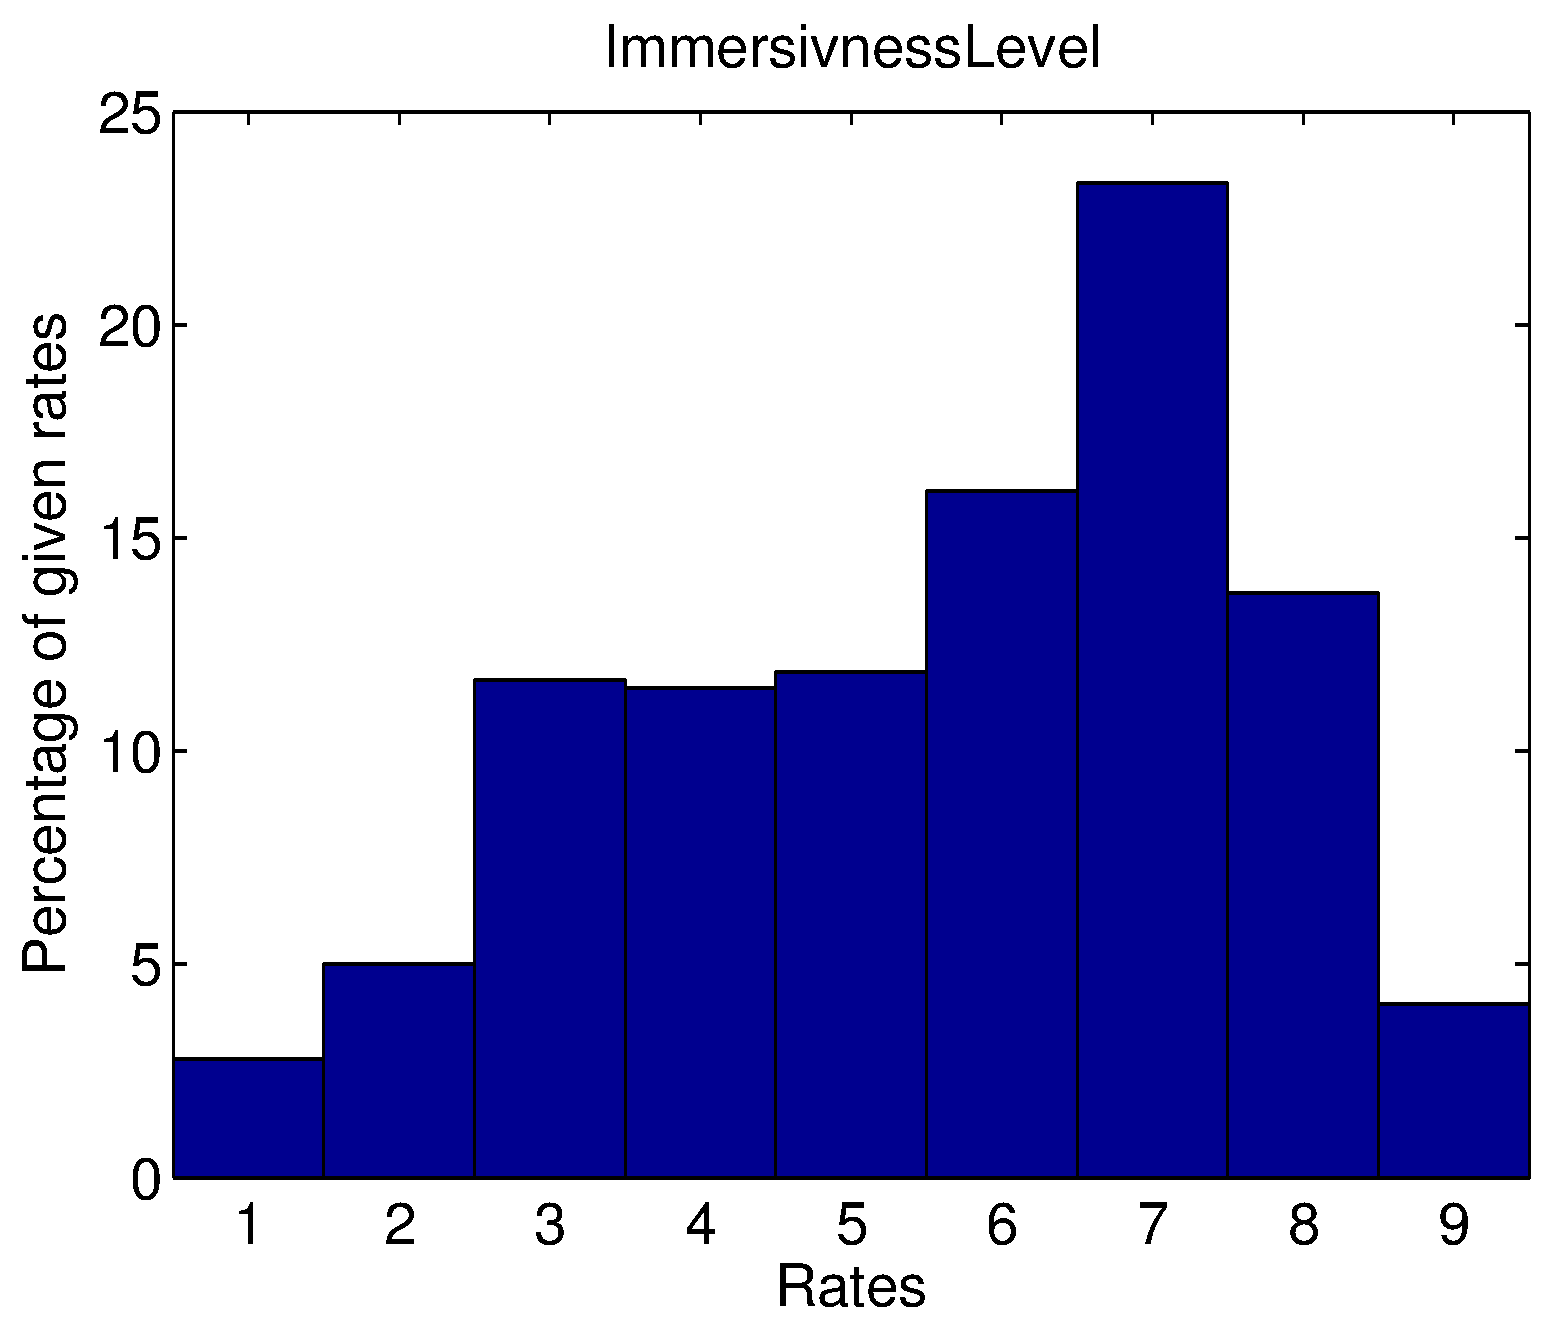
\includegraphics[width=0.3\textwidth]{./images/Hist9ImmersivnessLevel.png}
    \caption{Score distribution histogram for the \ac{IL} experienced }
    \label{Hist}
\end{figure}

As it can be observed all the \ac{IL} were experienced during the experiments. More specifically, the distribution of the rates is roughly 20\% for the three lowest \ac{IL}, 40\% for the three middle and highest \ac{IL}. Thus the distribution almost describes three classes of immersiveness.  

\indent Figure \ref{MOS} shows the resulting \ac{MOS} and \ac{CI} for the \ac{SoP} experienced during stimuli.
\begin{figure}[!ht]
    \center
    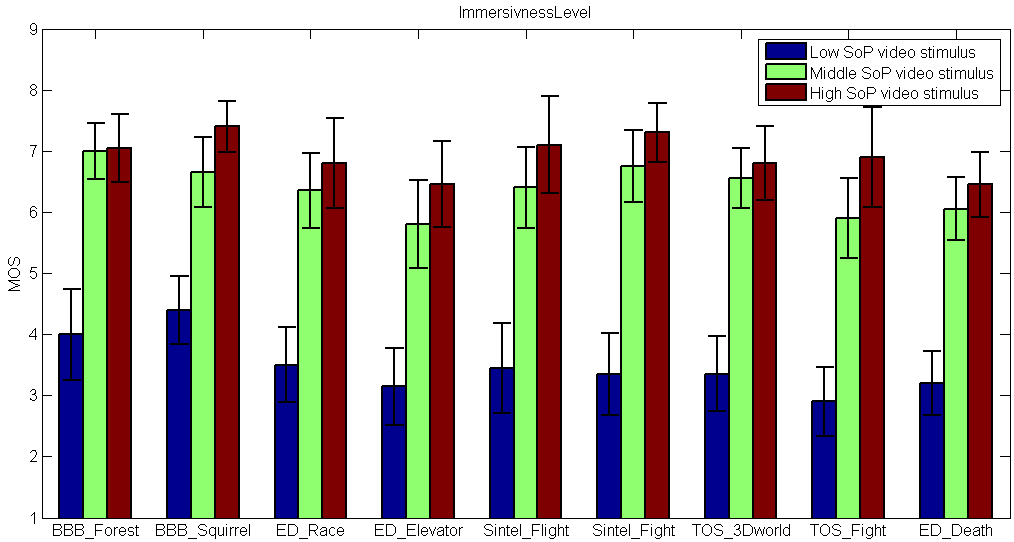
\includegraphics[width=0.4\textwidth]{./images/MOS_ImmersivnessLevel.png}
    \caption{\ac{MOS} and \ac{CI} for the \ac{IL} experienced}
    \label{MOS}
\end{figure}

The observed \ac{MOS} results valid the three \ac{IL} chosen during the experiment design. In fact, the low \ac{IL} is assessed around the rate 4, the middle \ac{IL} at about 6.5 and the high \ac{IL} at roughly 7. The high \ac{IL} is always better perceived than the middle one. This latter is also always better perceived than the low \ac{IL}.
However, the difference between the middle and high levels is not significant as the \ac{CI} considerably overlap for all contents.
Nevertheless the \ac{CI} attests that there is a high difference between the low \ac{IL} and the two other levels. Thus a study of immersiveness or non immersiveness \ac{QoE} is possible thanks to that database.

\indent To understand the impact of \ac{QoS} factors - such as the interest of the video and audio content, the quality and resolution of the video - and verify that the surrounding awareness is inversely related with the \ac{IL}, the correlation between the \ac{MOS} for all five factors was measure thanks to Pearson correlation coefficient. Figure \ref{Correlation} and Table \ref{OC} illustrate and report respectively how highly the \ac{IL} is correlated with the video quality and the overall correlation coefficients.

\begin{figure}[!ht]
    \center
    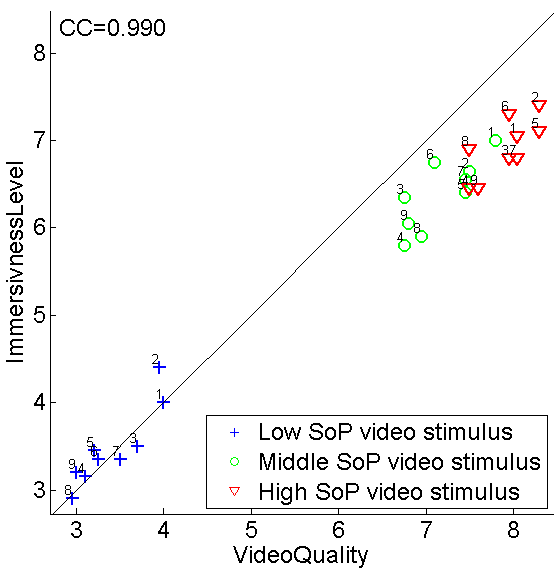
\includegraphics[width=0.3\textwidth]{./images/VA_IL_C.png}
    \caption{Correlation between the experienced \ac{SoP} and the assessed quality of the video }
    \label{Correlation}
\end{figure}

The figure \ref{Correlation} is the depiction of the correlation between the \ac{MOS} rates given for the video quality and the \ac{SoP}. Each sequence is identified by a number, allowing the study of the assessment evolution depending of the \ac{IL} of a sequence.
The correlation coefficient of \ac{IL} and video quality is 0.99, meaning that these two characteristics are highly correlated. A huge difference is observed between the low class and middle/high class, corroborating the previous analysis. It should be point out that each sequence provide a better immersive experience when its \ac{IL} is increased.


\begin{table}[h]
\resizebox{0.6\textwidth}{!}{
\begin{minipage}{0.7\textwidth}
\begin{tabular}{ |m{2cm} | m{1cm} m{2cm} m{2cm} m{1.6cm} | }
   %\hline	
   %frequency band of EEG features  \\
   \hline	
   		 	& video quality		& Interest in video content 	& Interest in audio content		& Surrounding awareness \\
   \hline	
   Immersiveness level 				& 0.990		& 0.914		& 0.974		& -0.986 \\
   video quality 					& 	-		& 0.892		& 0.988		& -0.987 \\
   Interest in video content 		& 	-		& 	-		& 0.857		& -0.903 \\
   Interest in audio content 		& 	-		& 	-		& 	-		& -0.965 \\
   \hline	
 \end{tabular}
\caption{Pearson correlation coefficients between the ratings of different perceptual aspects }
\label{OC}
\end{minipage} }
\end{table}

The table \ref{OC} confirms the high correlation between \ac{IL} and the video quality (cc = 0.99), and shows the influence to having sound or not (cc = 0.97). It also valid that the surrounding awareness is inversely related with the \ac{IL} (cc ~= -0.99).


\subsection{Physiological signal analysis}
This section presents the pre-processing steps to remove the artifacts, the feature extraction methods and the classification results.

\subsubsection{Pre-processing}
The manually rejection of muscle activity related \ac{EEG} electrodes leads to a total of 216 electrodes for processing and analysis. \ac{EEG} signals were filtered between 3-47 Hz using a third-order Butterworth filter, in order to remove \ac{EOG}and \ac{EMG} artifacts.
[TO SET : DENOISING FUNCTION]

\ac{ECG} signals were used to extract the \ac{HRV}, which reflects the sympathetic/parasympathetic modulation. \ac{HRV} is the physiological measurement of variation in the time interval between consecutive hearts beats.\\
In order to extract the \ac{HRV}, the interval between two QRS complexes defined as R-R interval ($t_{R-R}$)was estimated using the real-time algorithm developed by Pan and Tompkins \cite{HR}. Then the heart rate (HR, in beats per minute) was estimated as :
\begin{equation}
	HR = \frac{60}{t_{R-R}}
\end{equation}

The \ac{HRV} is the variation of HR over time. As the HR is a time-series of non-uniform R-R intervals, the HR was regularly resampled at 4 Hz rate.
[TO SET : respiration denoising]

Both respiratory signals (abdomen and thoracic) were filtered by a wavelet multivariate de-noising
\cite{waveletDenoise}.
It combines univariate wavelet de-noising in the basis where the estimated noise covariance matrix is diagonal and non-centered Principal Component Analysis (PCA) on approximations in the wavelet domain.

In the presented results, only 19 \ac{EEG} signals were kept to expedite the validation of the database.


\subsubsection{Feature extraction}
[He?]
\subsubsection{Classification}
[He?]

\subsubsection{Results}
[Me]


